\section{Результаты}
\newcommand{\evenCHCSystem}{\begin{varexampleblock}[0.83\textwidth]{Система дизъюнктов \onslide<2->{как формула свободной теории}}
    \begin{align*}
    \top&\rightarrow even(Z)\onslide<2->{)\land} \\
    \onslide<2->{\forall y. (}even(y) &\rightarrow even(S(S(y)))\onslide<2->{)\land} \\
    \onslide<2->{\forall x. (}even(x) \land even(S(x)) &\rightarrow \bot\onslide<2->{)}
    \end{align*}
\end{varexampleblock}}

\newcount\rPos
\newcount\modelFloat

\begin{frame}{\textbf{Результат 1.} Предложен метод вывода регулярных инвариантов при помощи поиска конечных моделей и доказана его корректность}
\only<1>{\framesubtitle{\textbf{Этап 1.} Устранить АТД ограничения при помощи унификации и введения новых дизъюнктов}}
\only<2>{\framesubtitle{\textbf{Этап 2.} Трансформировать систему в формулу свободной теории введением логических связок}}
\only<3-4>{\framesubtitle{\textbf{Этап 3.} Передать формулу в сторонний инструмент поиска конечных моделей}}
\only<5->{\framesubtitle{\textbf{Этап 4.} По конечной модели построить автомат над деревьями}}

\centering
\begin{tikzpicture}[remember picture, overlay]
\node<-3>[text width=\textwidth] (evenCHCs) at (-0.32,1.8) {\evenCHCSystem{}};
\onslide<1>{\calloutquote[width=7.8cm,position={(-1,0.7)},bubblePosition={(0,-0.5)},callout pointer width=.4cm,fill=yellow!60,rounded corners]{\Large АТД ограничения устранены}}
\node<3-4>[inner sep=0pt] (fmfinder) at (0.3,-1.8) {
\includegraphics[width=.52\textwidth,height=.28\textwidth]{resources/blender.png}};
\node<3-4> (fmfinderName) [above left=-39mm and -58mm of fmfinder,align=center,text width=50mm] {{\large Инструмент поиска конечных моделей}};
\node<3-> (leftpath) [above left=17mm and 0.1cm of fmfinder] {};
\node<3-> (rightpath) [above right=17mm and -0.5cm of fmfinder] {};
\node<3-4> (modelStart) [below=20mm of evenCHCs] {};
\draw<3>[->] (evenCHCs) edge (modelStart) {};
\node<4-> (model) [text width=\textwidth] at (leftpath) {\begin{varblock}[0.5\textwidth]{}
\begin{align*}
    \mathattention<5>{\domain{Nat}}&\mathattention<5>{=\{0,1\}}\\
    \mathattention<6>{\mystructur(Z)}&\mathattention<6>{=0}\\
    \mathattention<7>{\mystructur(S)(x)}&\mathattention<7>{=1-x}\\
    \mathattention<8>{\mystructur(even)}&\mathattention<8>{=\{0\}}
\end{align*}
\end{varblock}};
\node<3-> (modelEnd) [right=10mm of leftpath] {};
\draw<4>[->] (modelStart) |- (modelEnd);
\onslide<9>{\node[overlay,draw,fill=green!40,opacity=0.95,rounded rectangle,minimum height=15mm,minimum width=15cm,align=center] at (0, -1) {Язык построенного автомата является регулярным инвариантом исходной системы\\$\invariant(even) = \langOf{\automat} = \{ S^{2n}(Z) \mid n \geq 0 \}$};}
\onslide<5->{\node<5-> (automaton) at (rightpath) {
\begin{minipage}{.3\textwidth}
\begin{varblock}[\textwidth]{}
\begin{center}
\vphantom{\begin{tikzpicture}[shorten >=1pt,node distance=2cm,on grid,auto]
    \node[state,initial,initial text=$Z$,accepting] (s0) {$0$};
    \node[state] (s1) [right=of s0] {$1$};
    \path[->]
        (s0)    edge [bend left=25] node {$S$}       (s1)
        (s1)    edge [bend left=25] node {$S$}       (s0)
    ;
\end{tikzpicture}}\hspace*{-12mm}\raisebox{9mm}{
\begin{tikzpicture}[remember picture,overlay,shorten >=1pt,node distance=2cm,on grid,auto]
    \node[state,onslide=<6->{initial,initial text=$Z$},onslide=<8->{accepting}] (s0) {$0$};
    \node[state] (s1) [right=of s0] {$1$};
    \path<7->[onslide=<7->,->]
        (s0)    edge [bend left=25] node {$S$}       (s1)
        (s1)    edge [bend left=25] node {$S$}       (s0)
    ;
\end{tikzpicture}}
\end{center}
\end{varblock}
\end{minipage}};}
\end{tikzpicture}
\end{frame}

\begin{frame}{\textbf{Результат 2.} Предложен метод вывода синхронных регулярных инвариантов при помощи поиска конечных моделей}
\only<2>{\framesubtitle{\textbf{Этап 1.} Устранить АТД ограничения при помощи унификации и введения новых дизъюнктов}}
\only<3>{\framesubtitle{\textbf{Этап 2.} Построить декларативное описание синхронного автомата, выражающего инвариант системы}}
\only<4>{\framesubtitle{\textbf{Этап 3.} Передать формулу в сторонний инструмент поиска конечных моделей}}
\only<5>{\framesubtitle{\textbf{Этап 4.} По конечной модели построить автомат над деревьями}}
\begin{columns}
\begin{column}{0.49\textwidth}
\vspace*{-8pt}
\begin{exampleblock}{Регулярные языки не позволяют представлять синхронные отношения}
\small\vspace*{-10pt}
\begin{align*}
    \top &\rightarrow lt(Z, S(x))\\
    lt(x, y) &\rightarrow lt(S(x), S(y))\\
    lt(x, y) \land lt(y, x) &\rightarrow \bot
\end{align*}
\end{exampleblock}
\end{column}
\begin{column}{0.48\textwidth}
\onslide<3->{
\begin{exampleblock}{Декларативное описание синхронного автомата}
\small\vspace*{-10pt}
\begin{align*}
&R(q) \rightarrow R(p(d(f,g, q), d(f, g, q)))\\
&R(p(q_1, q_2)) \rightarrow \big(F(q_1) \rightarrow F(d(S, S, q_2))\big)\\
&\dots
\end{align*}
\end{exampleblock}}
\end{column}
\end{columns}
\onslide<5->{
\vspace*{-15pt}
\begin{varexampleblock}[\textwidth]{Из модели можно извлечь определение синхронного автомата $$A = \sautomaton{0, 1}{2}{1}$$}
\small\vspace*{-10pt}
\begin{align*}
\tuple{Z, Z} &\mapsto 0 &Z &\mapsto 0 &S(q) &\mapsto 0\\
\tuple{Z, S}(q) &\mapsto 1 &\tuple{S, Z}(q) &\mapsto 0 &\tuple{S, S}(q) &\mapsto q
\end{align*}
$$\langOf{A} = \left\{ \tuple{S^n(Z), S^m(Z)} \mid n < m \right\}$$
\end{varexampleblock}
}
\end{frame}

\begin{frame}{\textbf{Результат 3.} Предложен новый класс инвариантов, основанный на булевой комбинации элементарных и регулярных инвариантов}
Новый класс \emph{комбинированных инвариантов} представляется формулами вида:
$$\phi \Coloneqq \overline{t}\in \langOf{A} \mid t = t' \mid \neg\psi \mid \psi \land \psi' \mid \psi \lor \psi'$$
\vspace*{-8mm}
\begin{itemize}
    \item $\overline{t}\in \langOf{A}$~--- принадлежность кортежа термов регулярном языку автомата $A$
\end{itemize}
% \begin{tikzpicture}
% \node[draw,fill=green!40,opacity=0.95,rounded rectangle,minimum height=2cm,align=center] at (-1,0) {\begin{minipage}{80mm}$$\phi \Coloneqq \overline{x}\in \langOf{A} \mid t = t' \mid \neg\psi \mid \psi \land \psi' \mid \psi \lor \psi'$$\end{minipage}};
% \end{tikzpicture}
\end{frame}

\begin{frame}{\textbf{Результат 4.} Предложен метод совместного вывода инвариантов в этом классе посредством вывода инвариантов в подклассах}
\whenFullCompile{\centering\ciciPic}
\end{frame}

\begin{frame}{\textbf{Результат 5.} Проведено теоретическое сравнение рассмотренных классов инвариантов}
\framesubtitle{\textcolor{myResult}{Зелёным} выделены мои результаты; \textcolor{trivialResult}{фиолетовым}~--- результаты с тривиальным доказательством}
\begin{table}
\scriptsize
\begin{tabular}{| m{31mm} || c | c | c | c | c | c |}
\hline
\diagbox[width=35mm]{Свойство}{Класс} & \elemclass{} & \sizeelemclass{} & \regclass{} & \syncRegFlatClass{} & \syncRegFullClass{} & \regelemclass{} \\
\hline
Замкнут по $\cap$       & \itsTrivial{Да} & \itsTrivial{Да} & Да & \itsMyresult{Да} & \itsMyresult{Да} & \itsTrivial{Да} \\
Замкнут по $\cup$       & \itsTrivial{Да} & \itsTrivial{Да} & Да & \itsMyresult{Да} & \itsMyresult{Да} & \itsTrivial{Да} \\
Замкнут по $\setminus$       & \itsTrivial{Да} & \itsTrivial{Да} & Да & \itsMyresult{Да} & \itsMyresult{Да} & \itsTrivial{Да} \\
Разрешимо $\overline{t} \in I$          & Да & Да & Да & Да & \itsMyresult{Да} & Да \\
Разрешимо $I = \emptyset$    & Да & Да & Да & Да & \itsMyresult{Да} & Да\\
Выразимы рекурсивные отношения & \itsTrivial{Нет} & \itsTrivial{Частично} & \itsTrivial{Да} & \itsTrivial{Да} & \itsTrivial{Да} & \itsTrivial{Да} \\
Выразимы синхронные отношения & \itsTrivial{Да} & \itsTrivial{Да} & \itsTrivial{Нет} & \itsTrivial{Частично} & \itsTrivial{Да} & \itsTrivial{Да} \\
\hline
\end{tabular}
\end{table}
\begin{table}
\scriptsize
\centering
\begin{tabular}{| m{15mm} || x{13mm} | x{17mm} | x{10mm} | c | c | c |}
\hline
Класс & \elemclass{} & \sizeelemclass{} & \regclass{} & \syncRegFlatClass{} & \syncRegFullClass{} & \regelemclass{} \\
\hline
\elemclass{} & \itsTrivial$\emptyset$ & \itsTrivial$\emptyset$ & \itsMyresult\exLR{} & \itsMyresult\exLR{} & \itsMyresult\exLR{} & \itsTrivial$\emptyset$\\
\sizeelemclass{} & \itsTrivial$\infty$ & \itsTrivial$\emptyset$ & \itsMyresult\exLR{} & \itsMyresult\exLR{} & \itsMyresult\exLR{} & \itsMyresult\exLt{} \\
\regclass{} & \itsMyresult\exEvenLeft{} & \itsMyresult\exEvenLeft{} & \itsTrivial$\emptyset$ & \itsTrivial$\emptyset$ & \itsTrivial$\emptyset$ & \itsTrivial$\emptyset$\\
\syncRegFlatClass{} & \itsMyresult\exEvenLeft{} & \itsMyresult\exEvenLeft{} & \itsTrivial$\infty$ & \itsTrivial$\emptyset$ & \itsTrivial$\emptyset$ & \itsMyresult\exLt{}\\
\syncRegFullClass{} & \itsMyresult\exEvenLeft{} & \itsMyresult\exEvenLeft{} & \itsTrivial$\infty$ & \itsTrivial$\infty$ & \itsTrivial$\emptyset$ & \itsMyresult\exLt{}\\
\regelemclass{} & \itsTrivial$\infty$ & \itsMyresult\exEvenLeft{} & \itsTrivial$\infty$ & \itsMyresult\exLR{} & \itsMyresult\exLR{} & \itsTrivial$\emptyset$\\
\hline
\end{tabular}
\end{table}
\end{frame}

\begin{frame}{Реализация}
\begin{figure}[h]
% https://online.visual-paradigm.com/share.jsp?id=323637353533352d31
\centering
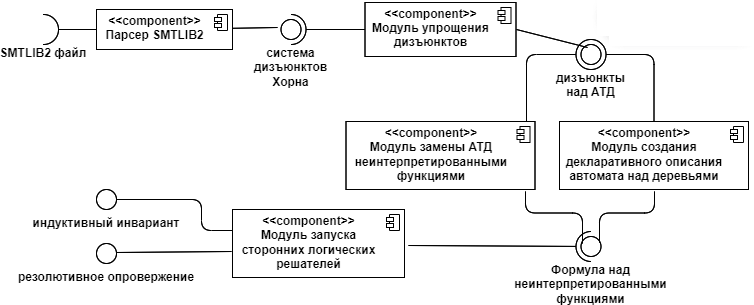
\includegraphics[width=\textwidth]{resources/arch.png}
\caption{Хорн-решатель \theringen{}: \url{https://github.com/Columpio/RInGen}}
% \label{fig:ringen-arch}
\end{figure}
\end{frame}

\begin{frame}{Сравнение Хорн-решателей с поддержкой АТД}
\begin{table}
\centering\footnotesize
% \caption{Сравнение Хорн-решателей с поддержкой АТД}\label{tab:hornSolvers}%
\begin{tabular}{| m{38mm} || x{18mm} | x{18mm} | x{18mm} | x{23mm} |}
% \hline
\hline
Инструмент & Класс\quad\ \ \  инвариантов & Метод & Возвращает инвариант & Полностью автоматический\\\hline\hline
\spacer{} & \elemclass{} & \pdr{} & Да & Да\\
\racer{} & \catelemclass{} & \pdr{} & Нет & Нет\\
\eldarica{} & \sizeelemclass{} & \cegar{} & Да & Да\\
\vericat{} & -- & Трансф. & Нет & Да\\
\hoice{} & \elemclass{} & \ice{} & Да & Да\\
\rchc{}  & \syncRegFlatClass{} & \ice{} & Да & Да\\\hline
\ringen{\cvc} & \regclass{} & Трансф. + \fmf{} & Да & Да\\
\ringen{\vampire} & -- & Трансф. + \satur{} & Нет & Да\\
\ringenSync{} & \syncRegFullClass{} & Трансф. + \fmf{} & Да & Да\\
\ringenCICI{\cvc} & \regelemclass{} & \ourCEGAR{} & Да & Да\\
\ringenCICI{\vampire} & -- & \ourCEGAR{} & Нет & Да\\
\hline
% \hline
\end{tabular}
\end{table}
\end{frame}

\begin{frame}{Эксперименты}
\vspace*{-10pt}
\begin{columns}
\begin{column}{.42\textwidth}
\begin{table}
% \caption{Результаты экспериментов. <<SAT>> обозначает, что система безопасна (есть индуктивный инвариант), <<UNSAT>> обозначает, что система небезопасна.}
% \label{table:eval-all}
\scriptsize
\centering
\begin{tabular}{ |l||c|c| }
\hline
Инструмент & SAT & UNSAT\\\hline\hline
\racer{} & 26 & 22\\
\eldarica{} & 46 & 12\\
\vericat{} & 16 & 10\\
\cvcind{} & 0 & 13\\
\hline
\ringen{\cvc{}} & 25 & 21\\
\ringen{\vampire{}} & 135 & 46\\
\ringenSync{} & 43 & 21\\
\ringenCICI{\cvc{}} & 117 & 19\\
\ringenCICI{\vampire{}} & 189 & 28\\
\hline
\end{tabular}
\end{table}
\end{column}
\begin{column}{.5\textwidth}
\pgfplotstableread[col sep = comma]{resources/experiments1.csv}\all
\begin{figure}[h]
\begin{center}
\begin{tikzpicture}[scale=0.55]
\begin{axis}[xmode=log, ymode=log, legend pos= north west, xlabel={Время работы \ringen{\cvc{}}, мс}, xlabel style = {align=center,font=\footnotesize}, ylabel style = {align=center,font=\footnotesize}, ylabel={Время работы {\color{red}\racer{}}, {\color{blue}\eldarica{}},\\{\color{brown}\cvcind{}} и {\color{cyan}\verimap{}}, мс}]
% \begin{axis}[xmode=log, ymode=log, legend pos= north west, xlabel={ Regular model construction by \theringen{}}, ylabel style = {align=center}, ylabel={Elementary model construction by \\{\color{red}\textsc{Spacer}}, {\color{blue}\eldarica{}} and {\color{brown}\cvcind{}}}]
    \addplot[dashed,no marks,very thin] coordinates {(10,10) (600000,600000)};
    \addplot [dashed, no marks, thin] coordinates {(10,10) (600000,600000)};
    \addplot [dashed, no marks, thin] coordinates {(10,300000) (300000,300000)};
    \addplot [dashed, no marks, thin] coordinates {(300000, 10) (300000,300000)};
    \addplot [dashed, no marks, thin] coordinates {(10, 600000) (600000,600000)};
    \addplot [dashed, no marks, thin] coordinates {(600000, 10) (600000,600000)};

    \addplot  [only marks,  mark=triangle, color=blue, mark size=3pt] table [x={CVC4Finite}, y={Eldarica}] {\all};
    \addplot  [only marks,  mark=o, color=red,  mark size=3pt] table [x={CVC4Finite}, y={Z3}] {\all};
    \addplot  [only marks,  mark=x, color=brown, mark size=3pt] table [x={CVC4Finite}, y={CVC4Ind}] {\all};
    \addplot  [only marks,  mark=square, color=cyan, mark size=3pt] table [x={CVC4Finite}, y={VeriMAP-iddt}] {\all};
\end{axis}

\end{tikzpicture}
    % \caption{Сравнение производительности инструментов. Каждая точка на графике представляет пару длительностей выполнения.}
% \label{fig:toolplotOne}
\end{center}
\end{figure}
\end{column}
\end{columns}
\vspace*{-5pt}
\begin{figure}
\toolplotTwo{\cvc{}}{resources/toolplot_cvc.csv}
~
\toolplotTwo{\vampire{}}{resources/toolplot_vampire.csv}
% \caption{Сравнение времени работы инструментов}
% \label{fig:toolplot}
\end{figure}
\end{frame}
